\documentclass{beamer}
\usetheme{Madrid}

\usecolortheme{seahorse}

\title{We Love Beamer}
\subtitle{Using Beamer}
\author{Shattik Islam Rhythm}
\institute[CSE, BUET]{Department of CSE, BUET}
\date{\today}

\begin{document}

\begin{frame} 
    \maketitle
\end{frame}

\begin{frame}{Outline} 
    \tableofcontents
\end{frame}

\section{Basics}

\begin{frame}{I am the TITLE}
    I am the FRAME. \pause I build up beamer presentations. \pause It is paused.
\end{frame}

\setbeamercovered{transparent}

\begin{frame}{List}

    \begin{itemize}
        \item Point 1 \pause 
        \item Point 2 \pause 
        \begin{itemize}
            \item part 2.1
            \item part 2.3
        \end{itemize} \pause 
        \item You are wondering where is part 2.2
        \item Mind reading!
        \end{itemize}

\end{frame}

\begin{frame}
    \frametitle{More Lists}
    \begin{enumerate}[I]
    \item<3-> Look at part 1
    \item<2-> Look at I
    \begin{itemize}
    \item<3-> Look at part 2
    \item<4-> Look at III
    \end{itemize}
    \item<5-> Nothing to see here, on to the next frame ...
    \item<1-2> Look at II
    \end{enumerate}
\end{frame}

\begin{frame}{Text Formatting}
    \textbf<2>{Mission Hexa}

    \textit<2-3>{Mission Hexa}

    \textsl<2>{Mission Hexa}

    \textrm<2>{Mission Hexa}

    \textsf<2>{Mission Hexa}

    \textcolor<2>{orange}{Mission Hexa}

    \alert<2>{Mission Hexa}

    \structure<2>{Mission Hexa}
\end{frame}

\begin{frame}{How to use description type lists} 
    \begin{description}
        \item[API] Application Programming Interface
        \item[LAN] Local Area Network
        \item[ASCII] American Standard Code for Information Interchange
    \end{description}
\end{frame} 

\section{Columns \& Table}

\begin{frame}
    \frametitle{Using Columns}
    \begin{columns}
    \column{0.25\textwidth}
    Look at the right column
    \column{0.5\textwidth}
    \begin{figure}
        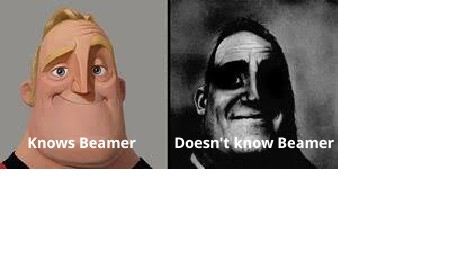
\includegraphics[width=\linewidth]{images.jpeg}
    \end{figure}
    \end{columns}
\end{frame}



\begin{frame} 
    \begin{table}
        \begin{tabular}{l | c | c | c | c }
        Competitor Name & Swim & Cycle & Run & Total \\
        \hline \hline
        John T & 13:04 & 24:15 & 18:34 & 55:53 \\ 
        Norman P & 8:00 & 22:45 & 23:02 & 53:47\\
        Alex K & 14:00 & 28:00 & n/a & n/a\\
        Sarah H & 9:22 & 21:10 & 24:03 & 54:35 
        \end{tabular}
        \caption{Triathlon results}
    \end{table}
\end{frame}


\begin{frame}
    \frametitle{Tables}
    \begin{table}
    \begin{tabular}{l | c | c | c | c }
    Competitor Name & Swim & Cycle & Run & Total \\
    \hline \hline
    John T & 13:04 & 24:15 & 18:34 & 55:53 \\ 
    \onslide<2-3> Norman P & 8:00 & 22:45 & 23:02 & 53:47 \\
    \onslide<3-> Alex K & 14:00 & 28:00 & n/a & n/a \\
    \onslide<4-> Sarah H & 9:22 & 21:10 & 24:03 & 54:35
    \onslide<1->
    \end{tabular}
    \caption{Triathlon results}
    \end{table}
\end{frame}

\section{Blocks}

\begin{frame}{Example of Blocks}

\begin{block}{Real Madrid}
    Greatest football club in the world. 
\end{block}

\begin{alertblock}{Surprising}
    Barcelona conceded 8 goals in one leg! 
\end{alertblock}

\begin{exampleblock}{UCL Titles}
    RMA has 15 titles!
\end{exampleblock}
    
\end{frame}

\begin{frame}{
    Math blocks
}
    \begin{theorem}[Pythagoras] 
    $ a^2 + b^2 = c^2$
    \end{theorem} \pause 
    \begin{corollary}
    $ x + y = y + x  $
    \end{corollary} \pause 
    \begin{proof}
    $\omega +\phi = \epsilon $
    \end{proof}    
\end{frame}

\end{document}